\section{Wstęp}

\begin{frame}{Plan prezentacji}
    \tableofcontents
\end{frame}

\begin{columnframe}{Motywacja}
    \begin{column}{0.5\textwidth}
        \begin{figure}
            \centering
            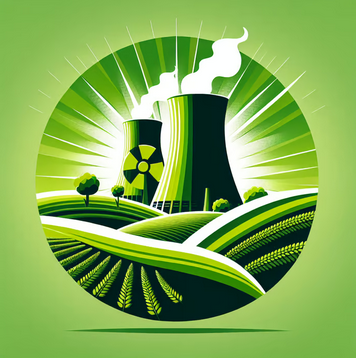
\includegraphics[width=0.8\textwidth, frame]{images/green_nuclear_stock.png}
        \end{figure}
    \end{column}
    \begin{column}{0.5\textwidth}
        \begin{itemize}
            \item Redukcja emisji CO2 i zanieczyszczeń
            \item Optymalizacja wykorzystania paliw kopalnych
            \item Zwiększenie stabilności i bezpieczeństwa energetycznego
        \end{itemize}
    \end{column}
\end{columnframe}

\begin{columnframe}{Czym jest SJW?}
    \begin{column}{0.5\textwidth}
        \begin{figure}
            \centering
            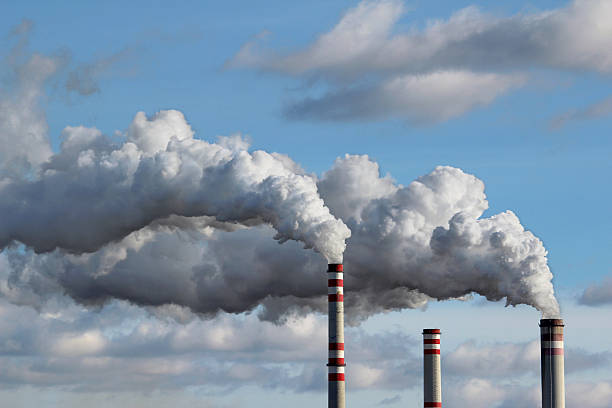
\includegraphics[width=0.9\textwidth, frame]{images/industrial_polution_stock_image.jpg}
        \end{figure}

        \begin{equation*}
            2\ch{H2O} \rightarrow 2\ch{H2} + \ch{O2}
        \end{equation*}

        \begin{equation*}
            \ch{CO2} \rightarrow \ch{C} + \ch{O2}
        \end{equation*}
        % \begin{equation*}
        %     \ch{CO2} + 4\ch{H2} \rightarrow \ch{CH4} + 2\ch{H2O}
        % \end{equation*}
    \end{column}
    \begin{column}{0.5\textwidth}
        \begin{itemize}
            \item Emisje CO2 stanowią problem ekologiczny
            \item Są sposoby na magazynowanie CO2 (lub jego wykorzywstanie w przemyśle chemicznym)
            \item Alternatywnie przestawianie atomów w cząsteczkach dwutlenku węgla i wody na inne związki
        \end{itemize}
    \end{column}
\end{columnframe}

\begin{columnframe}{Wyzwania wobec zmian klimatu}
    \begin{column}{0.5\textwidth}
        \begin{figure}
            \centering
            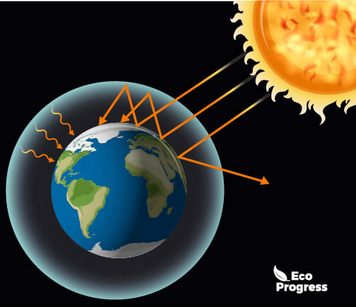
\includegraphics[width=0.8\textwidth, frame]{images/greenhouse_effect_stock_image.png}
        \end{figure}
    \end{column}
    \begin{column}{0.5\textwidth}
        Dwutlenek węgla (CO2) jest jednym z głównych gazów cieplarnianych, który odgrywa istotną rolę w zmianach klimatycznych. Wzrost jego stężenia w atmosferze przyczynia się do tzw. efektu cieplarnianego, czyli procesu, w którym gazy cieplarniane zatrzymują część promieniowania cieplnego Ziemi, zamiast pozwolić mu uciec w przestrzeń kosmiczną
    \end{column}
\end{columnframe}

\begin{frame}{Czym jest neutralność węglowa?}
    \begin{figure}
        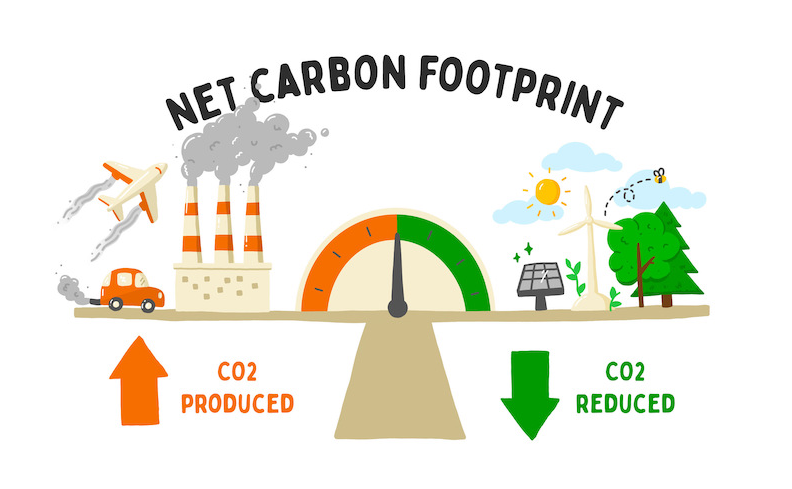
\includegraphics[width=0.7\textwidth]{images/carbon_footprint_infographic.png}
    \end{figure}



    Neutralność węglowa to stan, w którym emisje CO2 są równoważone przez ich pochłanianie lub redukcję (obecnie emitujemy więcej CO2 niż jesteśmy w stanie zatrzymać)
\end{frame}

\begin{frame}{Najwięksi emitenci CO2}
    \begin{figure}
        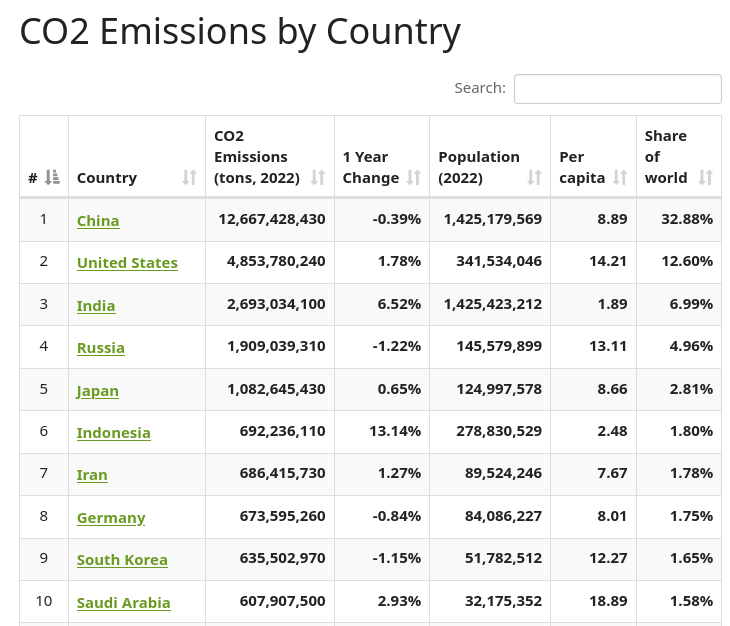
\includegraphics[width=0.7\textwidth]{images/top_polluters_table.png}
    \end{figure}
    Polska jest na 20-tym miejscu na świecie pod względem emisji CO2
\end{frame}

\begin{frame}{Emitenci CO2 w Polskim przemyśle}
    \begin{figure}
        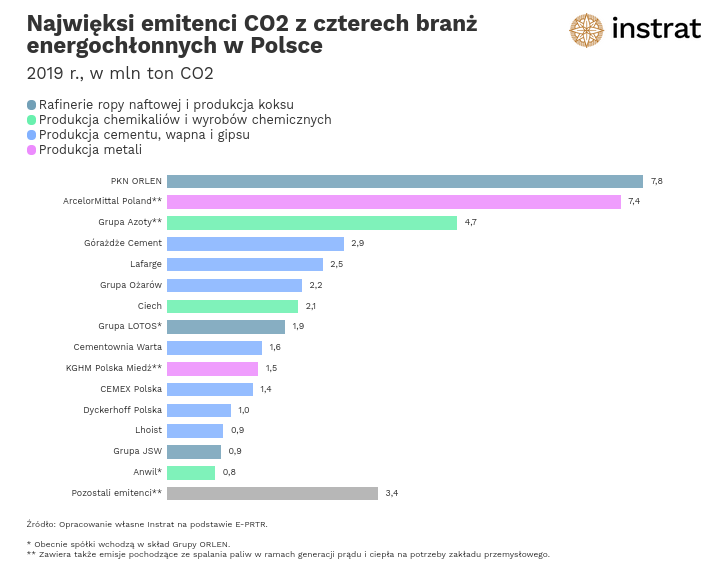
\includegraphics[width=0.8\textwidth]{images/top_polluters_poland.png}
    \end{figure}
\end{frame}


